%=============================================================================
% Relatorio Final INF2102 (Projeto Final de Programacao), DI PUC-Rio
% Explorador de Espaco Vetorial para Imagens
%=============================================================================

\documentclass[10pt]{article}
\usepackage[portuguese]{babel}

%=============================================================================
% PREÂMBULO
%=============================================================================

\title{Explorador de Espaço Vetorial para Imagens}

\usepackage[utf8]{inputenc}

\usepackage{amsmath}
\usepackage{amssymb}

\usepackage{graphicx}
\usepackage{color}
\usepackage{float}
\usepackage{capt-of}
\usepackage{caption}

\usepackage{anysize}
\marginsize{2cm}{2cm}{2cm}{2cm}
\usepackage{longtable}
\usepackage{booktabs}
\usepackage{array}

\usepackage[colorlinks=true,plainpages=true,citecolor=blue,linkcolor=blue,urlcolor=blue]{hyperref}

%=============================================================================
% CABEÇALHO E RODAPÉ
%=============================================================================

\usepackage{fancyhdr}
\pagestyle{fancy}
\fancyhf{}
\fancyhead[L]{\footnotesize Departamento de Informática}
\fancyhead[R]{\footnotesize PUC-Rio}
\fancyfoot[R]{\footnotesize INF2102}
\fancyfoot[C]{\thepage}
\fancyfoot[L]{\footnotesize Pós-Graduação, Mestrado em Informática}
\renewcommand{\footrulewidth}{0.4pt}
\fancypagestyle{firststyle}{\fancyhf{}}

%=============================================================================
% CÓDIGO FONTE (Python)
%=============================================================================

\usepackage{listings}
\definecolor{dkgreen}{rgb}{0,0.6,0}
\definecolor{gray}{rgb}{0.5,0.5,0.5}
\definecolor{mauve}{rgb}{0.58,0,0.82}
\definecolor{codebg}{rgb}{0.97,0.97,0.97}

\lstset{
   language=Python,
   basicstyle=\ttfamily\footnotesize,
   keywordstyle=\color{blue},
   commentstyle=\color{gray},
   stringstyle=\color{dkgreen},
   numberstyle=\tiny\color{gray},
   backgroundcolor=\color{codebg},
   frame=single,
   framesep=4pt,
   breaklines=true,
   showstringspaces=false,
   tabsize=2,
   columns=fullflexible,
}

%=============================================================================
% DOCUMENTO
%=============================================================================

\begin{document}

% Página de título
\thispagestyle{firststyle}
\begin{center}
  \begin{minipage}{0.48\textwidth}\begin{flushleft}
    
\includegraphics[scale=0.75]{images/di.png}
  \end{flushleft}\end{minipage}
  \begin{minipage}{0.48\textwidth}\begin{flushright}
    
\includegraphics[scale=0.4]{images/puc.png}
  \end{flushright}\end{minipage}

  \vspace*{1.5cm}

  \textsc{\LARGE Departamento de Informática}\\[1.5cm]
  \textsc{\LARGE INF2102: Projeto Final de Programação}\\[1.5cm]

  \vspace{0.5cm}
  \vspace*{1cm}

  {\huge\bfseries Explorador de Espaço Vetorial para Imagens}\\[0.4cm]
  \vspace*{1cm}
  {\large
    \vspace*{0.2cm}
    Gabriel Ribeiro Gomes \\ \texttt{ggomes@inf.puc-rio.br} \\[0.4cm]
    \vspace*{0.6cm}
    \emph{Orientador:} \\ Alberto Barbosa Raposo \\ \texttt{abraposo@inf.puc-rio.br}
  }

  \vspace{2cm}
  \begin{center}
    {Rio de Janeiro \\ Julho de 2026}
  \end{center}
\end{center}

\newpage

% O que é CBIR
\section{O que é Recuperação de Imagens por Conteúdo (CBIR)}

Recuperação de imagens por conteúdo (do inglês \emph{Content-Based Image
Retrieval}, CBIR) é a tarefa de buscar imagens semelhantes a uma imagem de
consulta usando o próprio conteúdo visual, e não texto, etiquetas ou metadados
associados. A ideia central: converter cada imagem em um vetor numérico (um
\emph{embedding}) que captura suas características visuais, de modo que imagens
parecidas fiquem próximas em um espaço vetorial e imagens diferentes fiquem
distantes. A busca por semelhança vira, então, uma busca por vizinhos mais
próximos nesse espaço.

Isso é importante por várias razões práticas e de pesquisa:

\begin{itemize}
  \item \textbf{Busca sem rótulos:} encontrar imagens relevantes mesmo quando
  não há descrição textual, o que é comum em grandes acervos não anotados.
  \item \textbf{Rotulagem automática:} se uma imagem nova cai perto de um
  aglomerado de imagens de classe conhecida, pode-se propor um rótulo para ela.
  Esse é o princípio que motiva este trabalho e a dissertação associada.
  \item \textbf{Avaliação de representações:} a qualidade de um \emph{embedding}
  pode ser julgada por quão bem ele agrupa imagens da mesma classe e separa
  classes diferentes.
\end{itemize}

O desafio central da área é obter representações que capturem semelhança
\emph{semântica}, e não apenas semelhança de pixels: duas fotos do mesmo objeto
sob ângulos ou iluminações diferentes devem ficar próximas. Modelos modernos de
visão (como CLIP) produzem embeddings genéricos fortes, e uma parte importante
da pesquisa em CBIR é justamente medir o quão confiáveis esses embeddings são
para uma tarefa concreta. Este programa serve exatamente a esse propósito:
tornar visível e mensurável o comportamento de recuperação.

\medskip
\noindent\textbf{Estudo de caso e dados de exemplo.} O sistema é genérico e
funciona com qualquer imagem. O conjunto de amostra usado nas demonstrações vem
de um projeto de monitoramento de embarcações na Baía de Guanabara (TecGraf
PUC-Rio / Embraer), mas nada no sistema é específico desse domínio.

% Breve Descrição
\section{Breve Descrição}

O \textbf{Explorador de Espaço Vetorial para Imagens} é uma ferramenta de
recuperação de imagens por conteúdo. O programa indexa \emph{embeddings} de
imagem em um banco de dados vetorial e permite \textbf{explorar visualmente o
espaço de representação}: projeta a galeria indexada em 2D/3D via PCA, aceita
uma imagem de consulta, e mostra onde ela se posiciona em relação aos
aglomerados (\emph{clusters}) de cada classe. Além disso, prevê por votação
\emph{K-Nearest Neighbors} (KNN) sobre os vizinhos recuperados a que classe a
imagem consultada pertenceria, com um grau de confiança.

\subsection*{Principais funções}

\begin{table}[H]
\centering
\begin{tabular}{@{}p{3.2cm}p{11cm}@{}}
\toprule
\textbf{Função} & \textbf{Descrição} \\
\midrule
Indexação & Extrai \emph{embeddings} de recortes de imagem com um modelo selecionável e os armazena no Milvus. \\
Projeção & Reduz os \emph{embeddings} da galeria a 2D/3D com PCA para visualização. \\
Consulta visual & Projeta uma imagem nova no \emph{mesmo} espaço da galeria e destaca seus vizinhos mais próximos. \\
Predição de classe & Vota, por KNN, a classe da imagem consultada e reporta a confiança. \\
Snapshot reproduzível & Exporta/reconstrói uma coleção a partir de um cache de \emph{embeddings} (sem GPU). \\
\bottomrule
\end{tabular}
\caption{Funções oferecidas pelo programa.}
\end{table}

\noindent\textbf{Usuários visados:} pesquisadores e estudantes de \emph{CBIR} /
visão computacional que precisam \textbf{conferir visualmente} se a recuperação
e a classificação de suas representações estão coerentes, em vez de confiar
apenas em métricas agregadas.

\medskip
\noindent\textbf{Natureza do programa:} ferramenta utilitária funcional (prova
de conceito madura), servindo de base experimental para uma dissertação de
mestrado sobre rotulagem automática por recuperação.

\medskip
\noindent\textbf{Ressalva de uso:} o programa \textbf{não} treina modelos e
\textbf{não} é um classificador de produção. A predição KNN é uma
\emph{heurística de rotulagem por recuperação}, cuja confiabilidade é justamente
o objeto de estudo. Os \emph{embeddings} vêm de um modelo genérico externo
(OpenCLIP), não de um modelo especializado no domínio.

% Visão de Projeto
\section{Visão de Projeto}

Esta seção apresenta quatro cenários (dois positivos e dois negativos) que
orientam a intenção do criador e a interpretação do usuário.

\subsection{Cenário Positivo 1: Conferir um agrupamento coerente}

Marina, pesquisadora de CBIR, quer saber se um \emph{embedding} genérico separa
bem recortes de \texttt{Traineira} de \texttt{Rebocador}. Ela indexa a galeria
de amostra, abre o explorador, escolhe a projeção 3D e vê quatro nuvens de cor
razoavelmente distintas. Ela arrasta um recorte de \texttt{Rebocador} como
consulta: o ponto vermelho cai \textbf{dentro} da nuvem de \texttt{Rebocador},
os 10 vizinhos exibidos são todos rebocadores, e o painel de predição mostra
\textbf{``seria rotulada como Rebocador, 90\% de confiança''}. Marina conclui,
visualmente, que a representação é adequada para essa classe naquela faixa de
tamanho.

\begin{quote}\small
Este cenário evoca as funções centrais: indexação, projeção, consulta e
predição. Note que Marina não precisou de nenhuma métrica agregada: a resposta
veio da posição do ponto e da concordância dos vizinhos.
\end{quote}

\subsection{Cenário Positivo 2: Trocar de modelo com garantia de consistência}

Pedro desconfia que \emph{patches} menores capturariam melhor embarcações
pequenas. Ele reindexa a mesma galeria com \texttt{openclip-vit-b-16} em uma
coleção separada. Ao abrir o explorador e selecionar essa coleção, a interface
exibe \textbf{``modelo de embedding: openclip-vit-b-16''} e garante que qualquer
consulta será \emph{embeddada} com esse mesmo modelo. Pedro compara as duas
projeções lado a lado e decide qual modelo separa melhor as classes, sem risco
de comparar vetores de espaços diferentes.

\begin{quote}\small
Este cenário evoca a troca de modelos e a \textbf{garantia de consistência}: a
coleção ``lembra'' com qual modelo foi construída, e o sistema recusa misturar
espaços de \emph{embedding}.
\end{quote}

\subsection{Cenário Negativo 1: Consulta com modelo incompatível}

Ana tenta, via API, consultar uma coleção construída com
\texttt{openclip-vit-b-32} forçando o modelo \texttt{openclip-vit-b-16}. O
sistema \textbf{recusa} a operação com um erro \texttt{409 Conflict} e a
mensagem: \emph{``a coleção foi construída com openclip-vit-b-32, mas a consulta
pediu openclip-vit-b-16; os embeddings seriam incomparáveis''}.

\begin{quote}\small
Este cenário ilustra uma limitação \textbf{conhecida e desejada}: distâncias
entre vetores de modelos diferentes não têm significado. O programa prefere
falhar de forma clara a devolver um resultado silenciosamente incorreto. Não há
como contornar isso pela interface, e é intencional.
\end{quote}

\subsection{Cenário Negativo 2: Recorte ambíguo mal classificado}

João consulta com um recorte de \texttt{Traineira} pequeno e distante, capturado
ao fundo de uma cena. O ponto de consulta cai na fronteira entre
\texttt{Traineira} e \texttt{Navio de Carga Geral}, e a predição KNN retorna
\textbf{``Navio de Carga Geral''} com alta confiança (um erro). Ao inspecionar
os vizinhos exibidos, João percebe que todos são embarcações pequenas e
distantes da mesma câmera: visualmente parecidas, apenas alguns \emph{pixels}.

\begin{quote}\small
Este cenário expõe uma limitação diferente da anterior: para objetos muito
pequenos, o \emph{embedding} genérico captura mais o contexto de cena do que o
objeto. O programa não esconde isso: ao contrário, a ferramenta \textbf{serve
exatamente para tornar esse tipo de falha visível}, o que é um resultado de
pesquisa, não um defeito de software.
\end{quote}

% Documentação Técnica
\section{Documentação Técnica do Projeto}

\subsection{Modelo de Arquitetura}

O sistema é organizado em três camadas com dependência unidirecional
(\emph{frontend} $\rightarrow$ API $\rightarrow$ \emph{backend}), mais os
contratos de dados e a observabilidade compartilhados
(Figura~\ref{fig:arch}).

\begin{figure}[H]
  \centering
  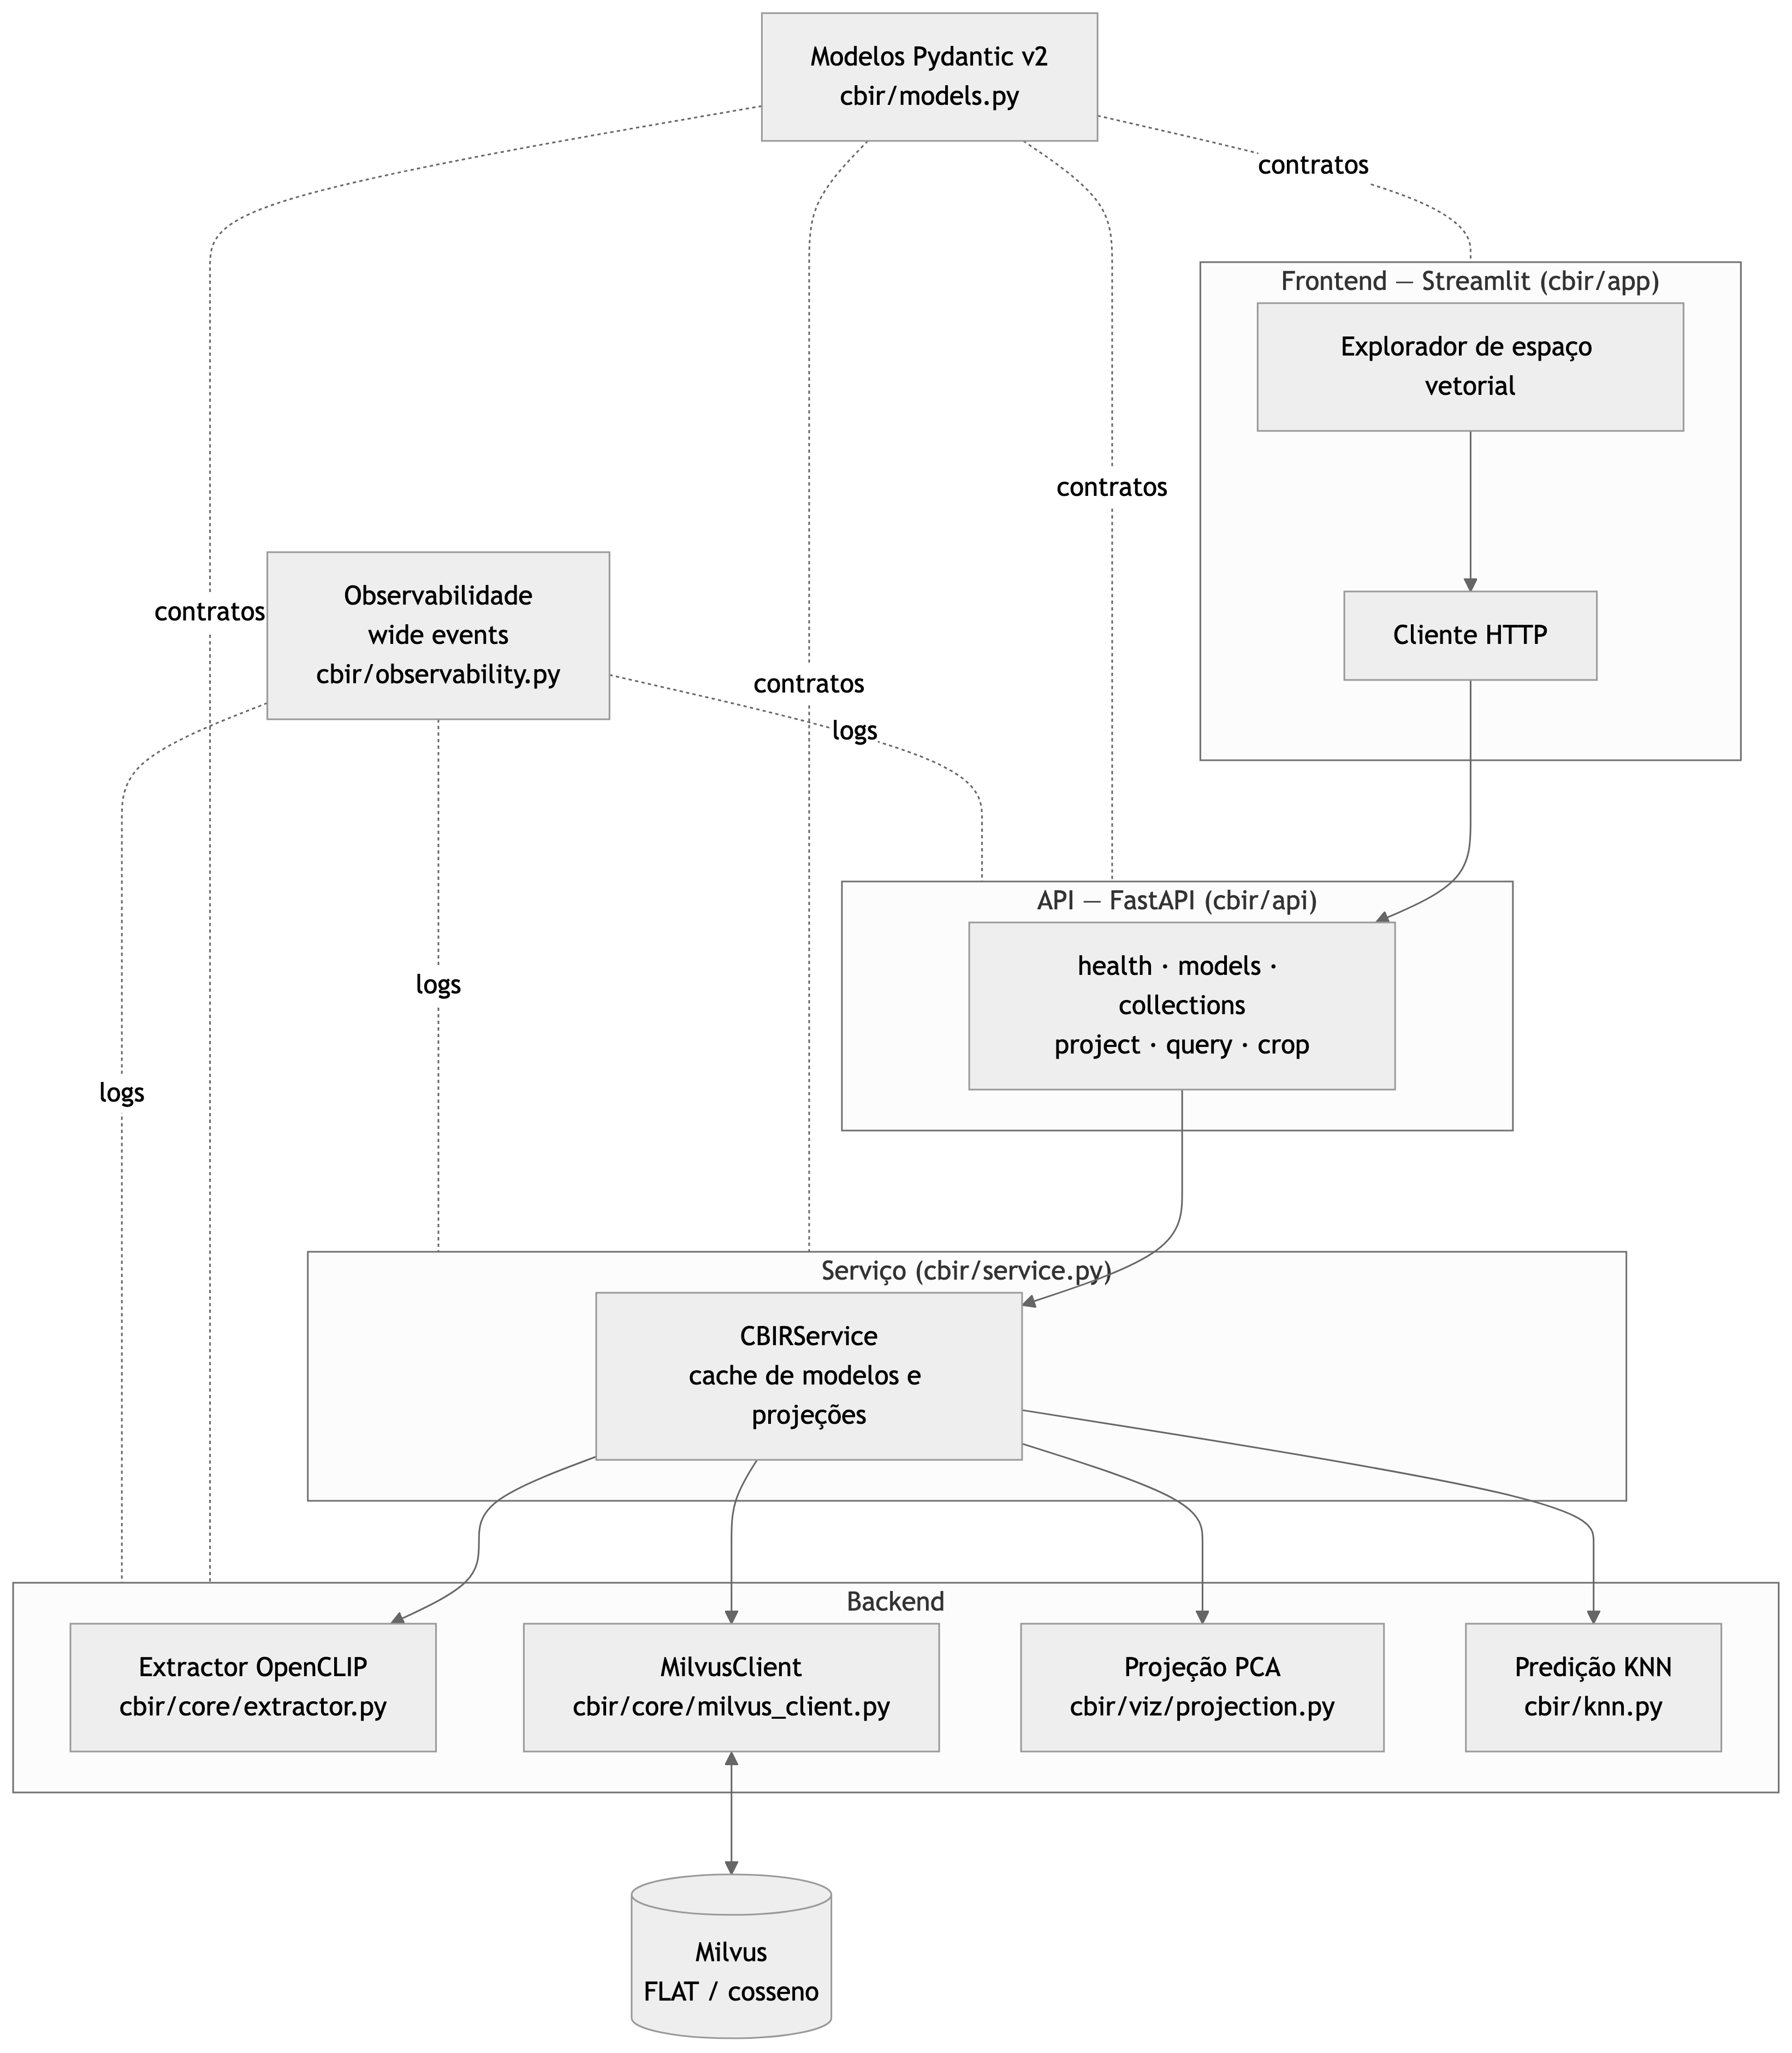
\includegraphics[width=0.82\textwidth]{images/arch.png}
  \caption{Arquitetura em três camadas. O \emph{frontend} fala apenas com a API;
  a API delega ao serviço; o serviço orquestra o \emph{backend} e o Milvus.}
  \label{fig:arch}
\end{figure}

\subsection{Modelo de Dados}

A unidade canônica é o \textbf{recorte de \emph{bounding box}}. Um
\emph{manifest} (JSONL, um registro por caixa) descreve cada item; o recorte é
derivado em tempo de execução. Os \emph{embeddings} e metadados são persistidos
no Milvus. A Figura~\ref{fig:classes} apresenta as classes principais e a
Figura~\ref{fig:er} o diagrama entidade-relação das entidades persistidas.

\begin{figure}[H]
  \centering
  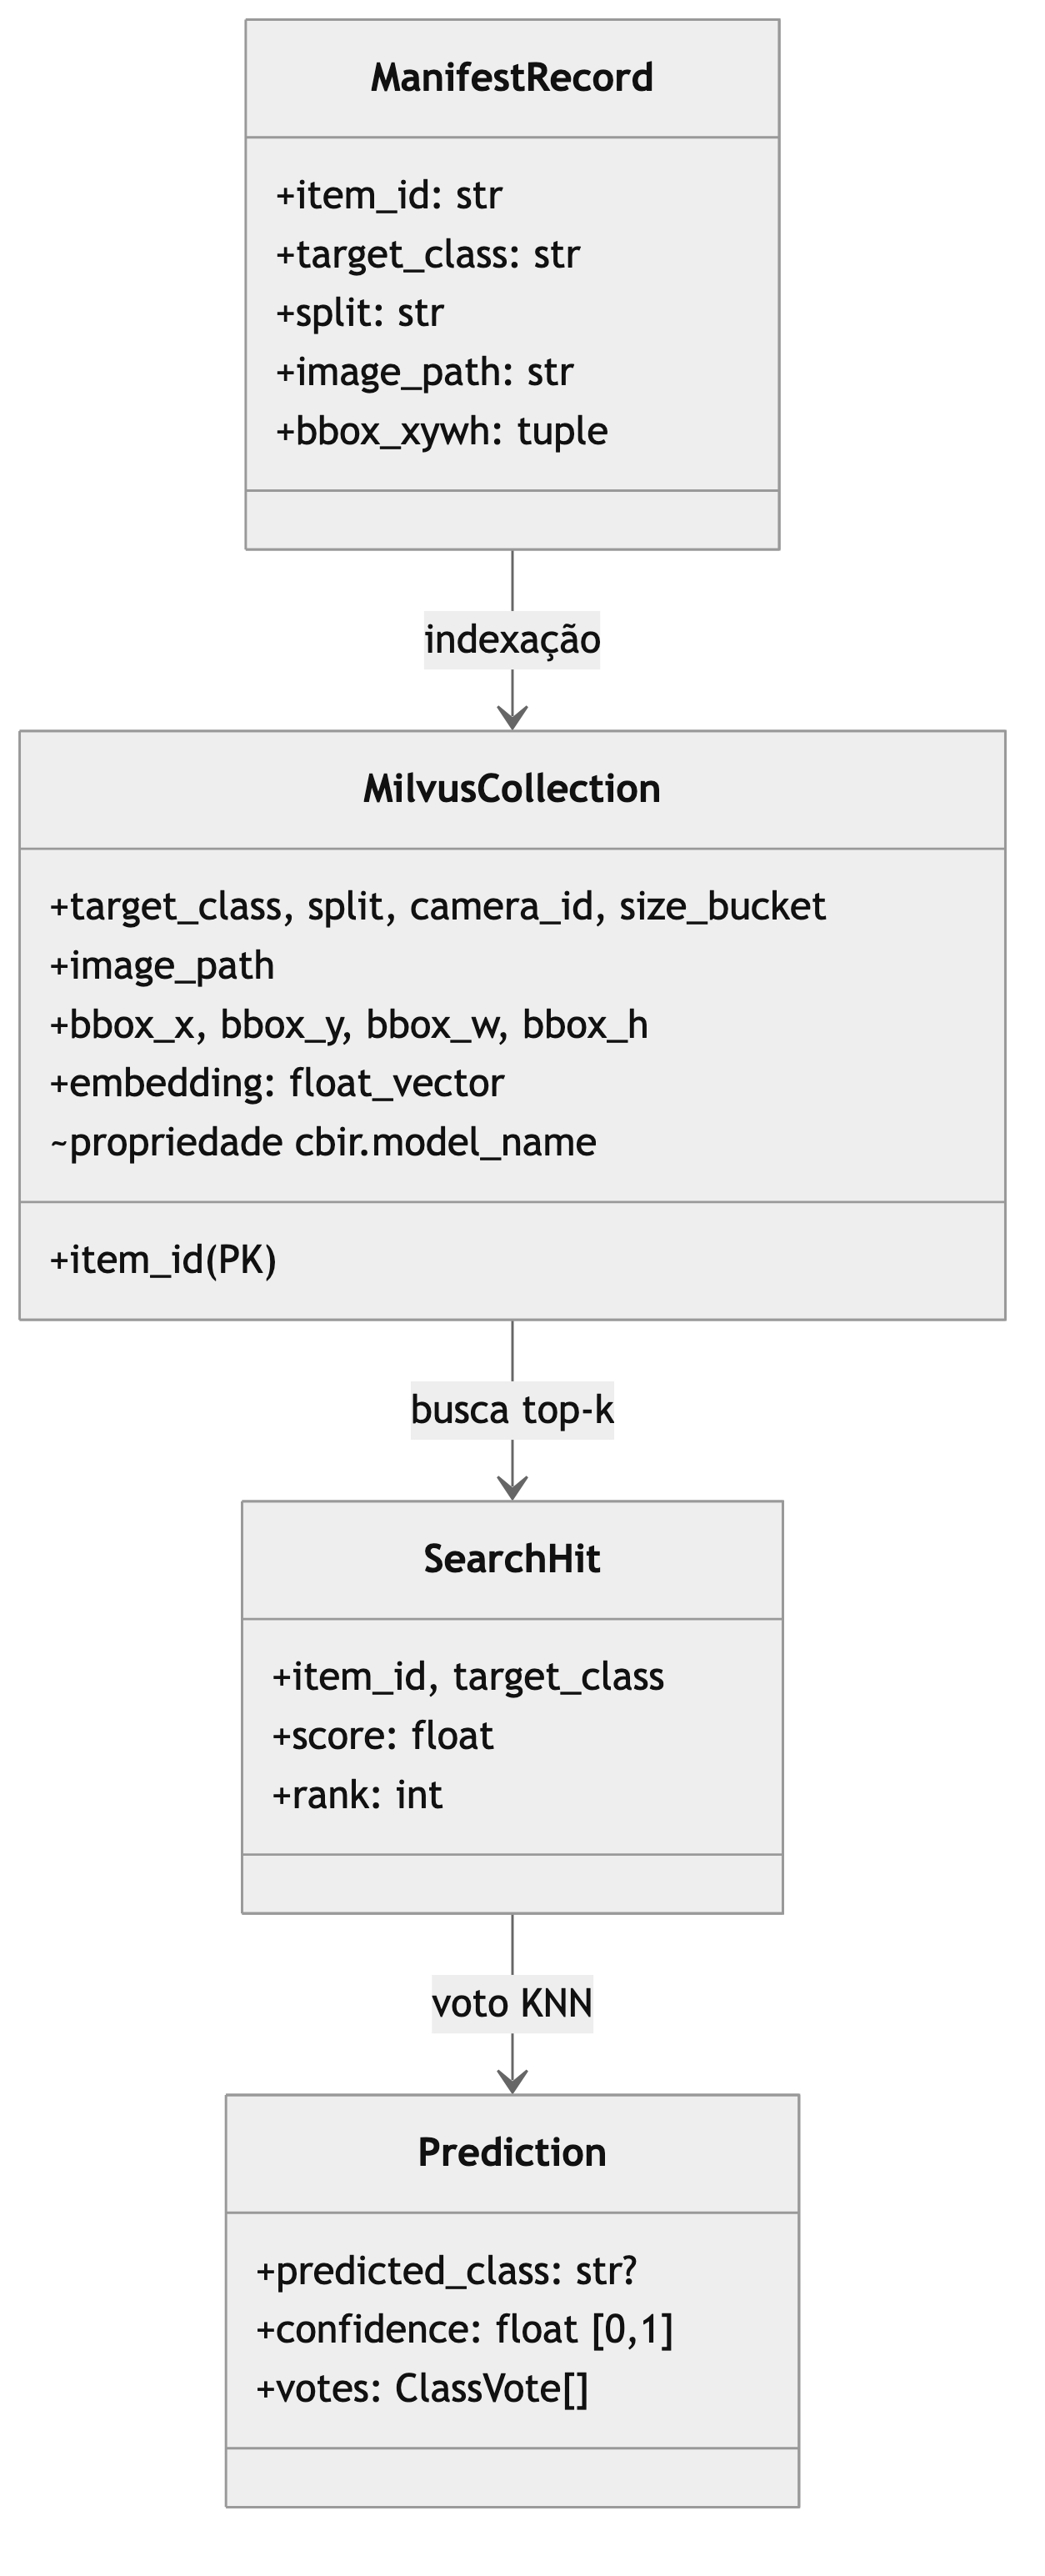
\includegraphics[height=0.34\textheight]{images/classes.png}
  \caption{Principais classes de dados (contratos Pydantic v2).}
  \label{fig:classes}
\end{figure}

\begin{figure}[H]
  \centering
  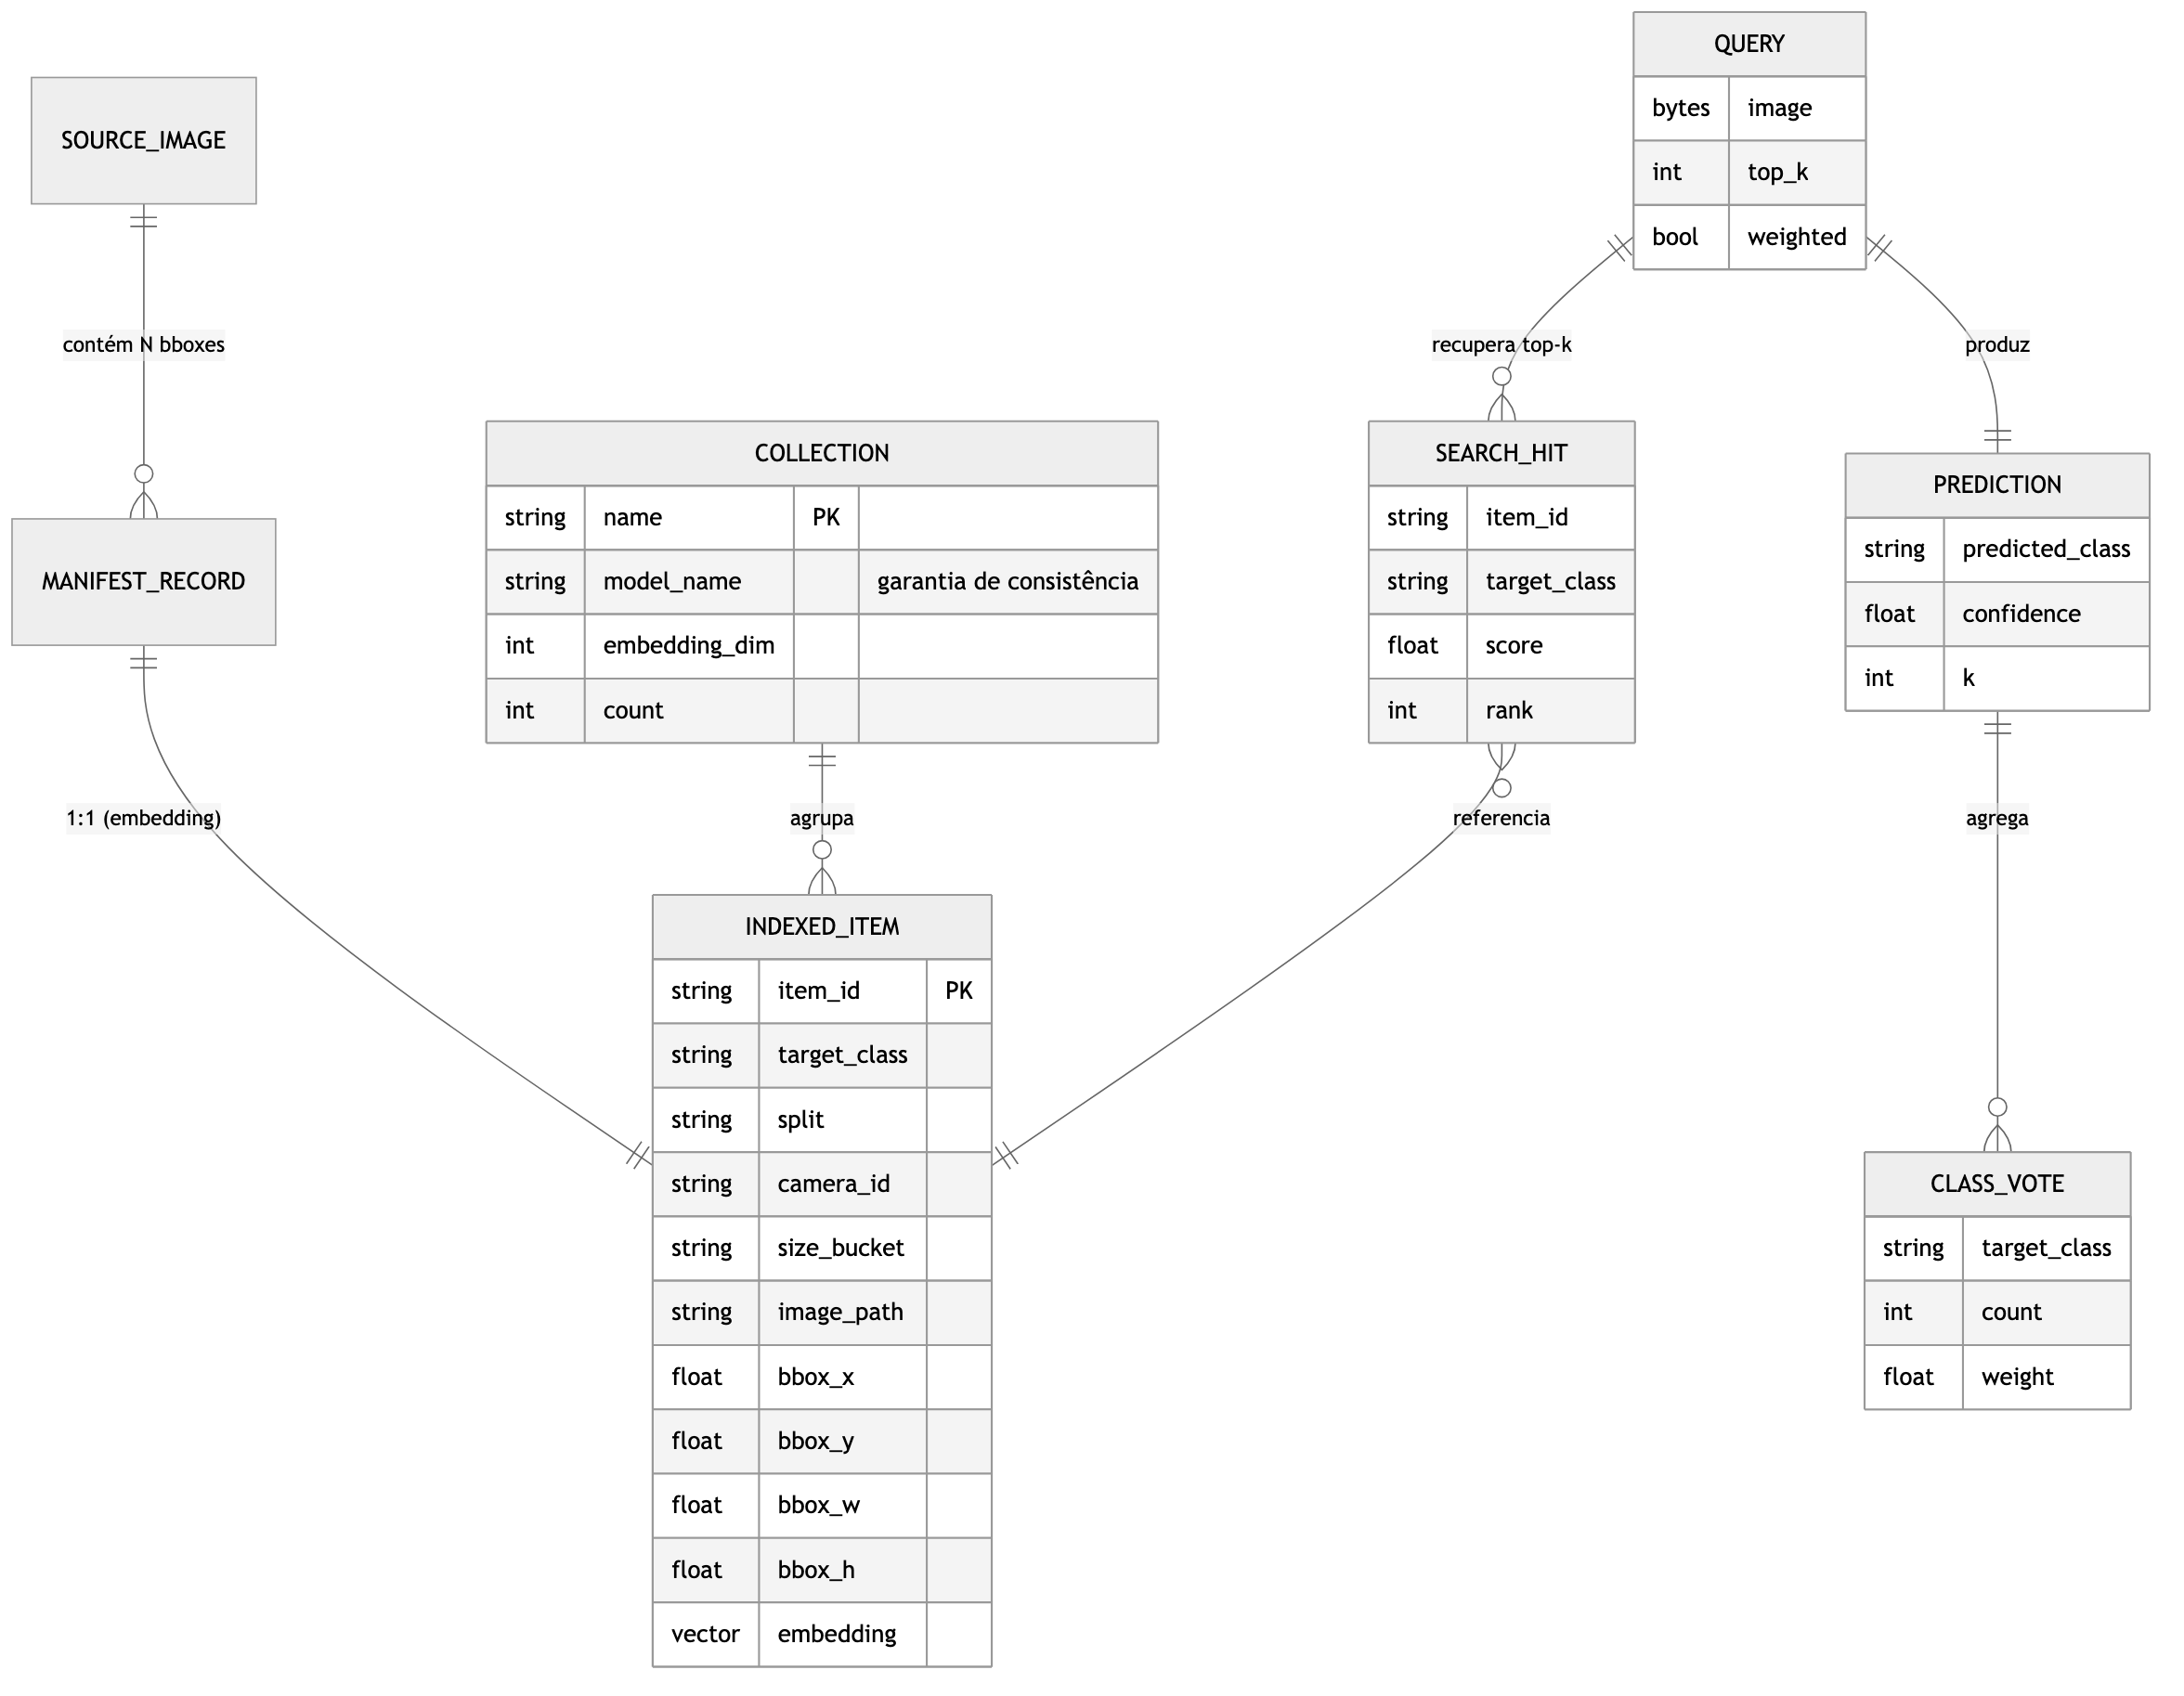
\includegraphics[width=0.92\textwidth]{images/er.png}
  \caption{Diagrama entidade-relação. Uma imagem-fonte contém $N$ caixas; cada
  caixa vira um item indexado; cada consulta recupera $k$ vizinhos, que alimentam
  uma predição.}
  \label{fig:er}
\end{figure}

O esquema de metadados carregado com cada vetor foi escolhido para ser
exatamente o que o \emph{frontend} precisa:

\begin{table}[H]
\centering
\begin{tabular}{@{}p{4cm}p{10cm}@{}}
\toprule
\textbf{Campo} & \textbf{Uso} \\
\midrule
\texttt{target\_class} & Cor do ponto no gráfico e voto KNN \\
\texttt{split}, \texttt{camera\_id}, \texttt{size\_bucket} & Facetas / \emph{hover} \\
\texttt{image\_path} & Servir o recorte como miniatura \\
\texttt{bbox\_x..h} & Reconstruir o recorte quando necessário \\
\texttt{embedding} & Vetor para busca por cosseno \\
\emph{propriedade} \texttt{cbir.model\_name} & \textbf{Garantia de consistência de modelo} \\
\bottomrule
\end{tabular}
\caption{Esquema de metadados por vetor na coleção Milvus.}
\end{table}

\subsection{Fluxo de Indexação}

\begin{figure}[H]
  \centering
  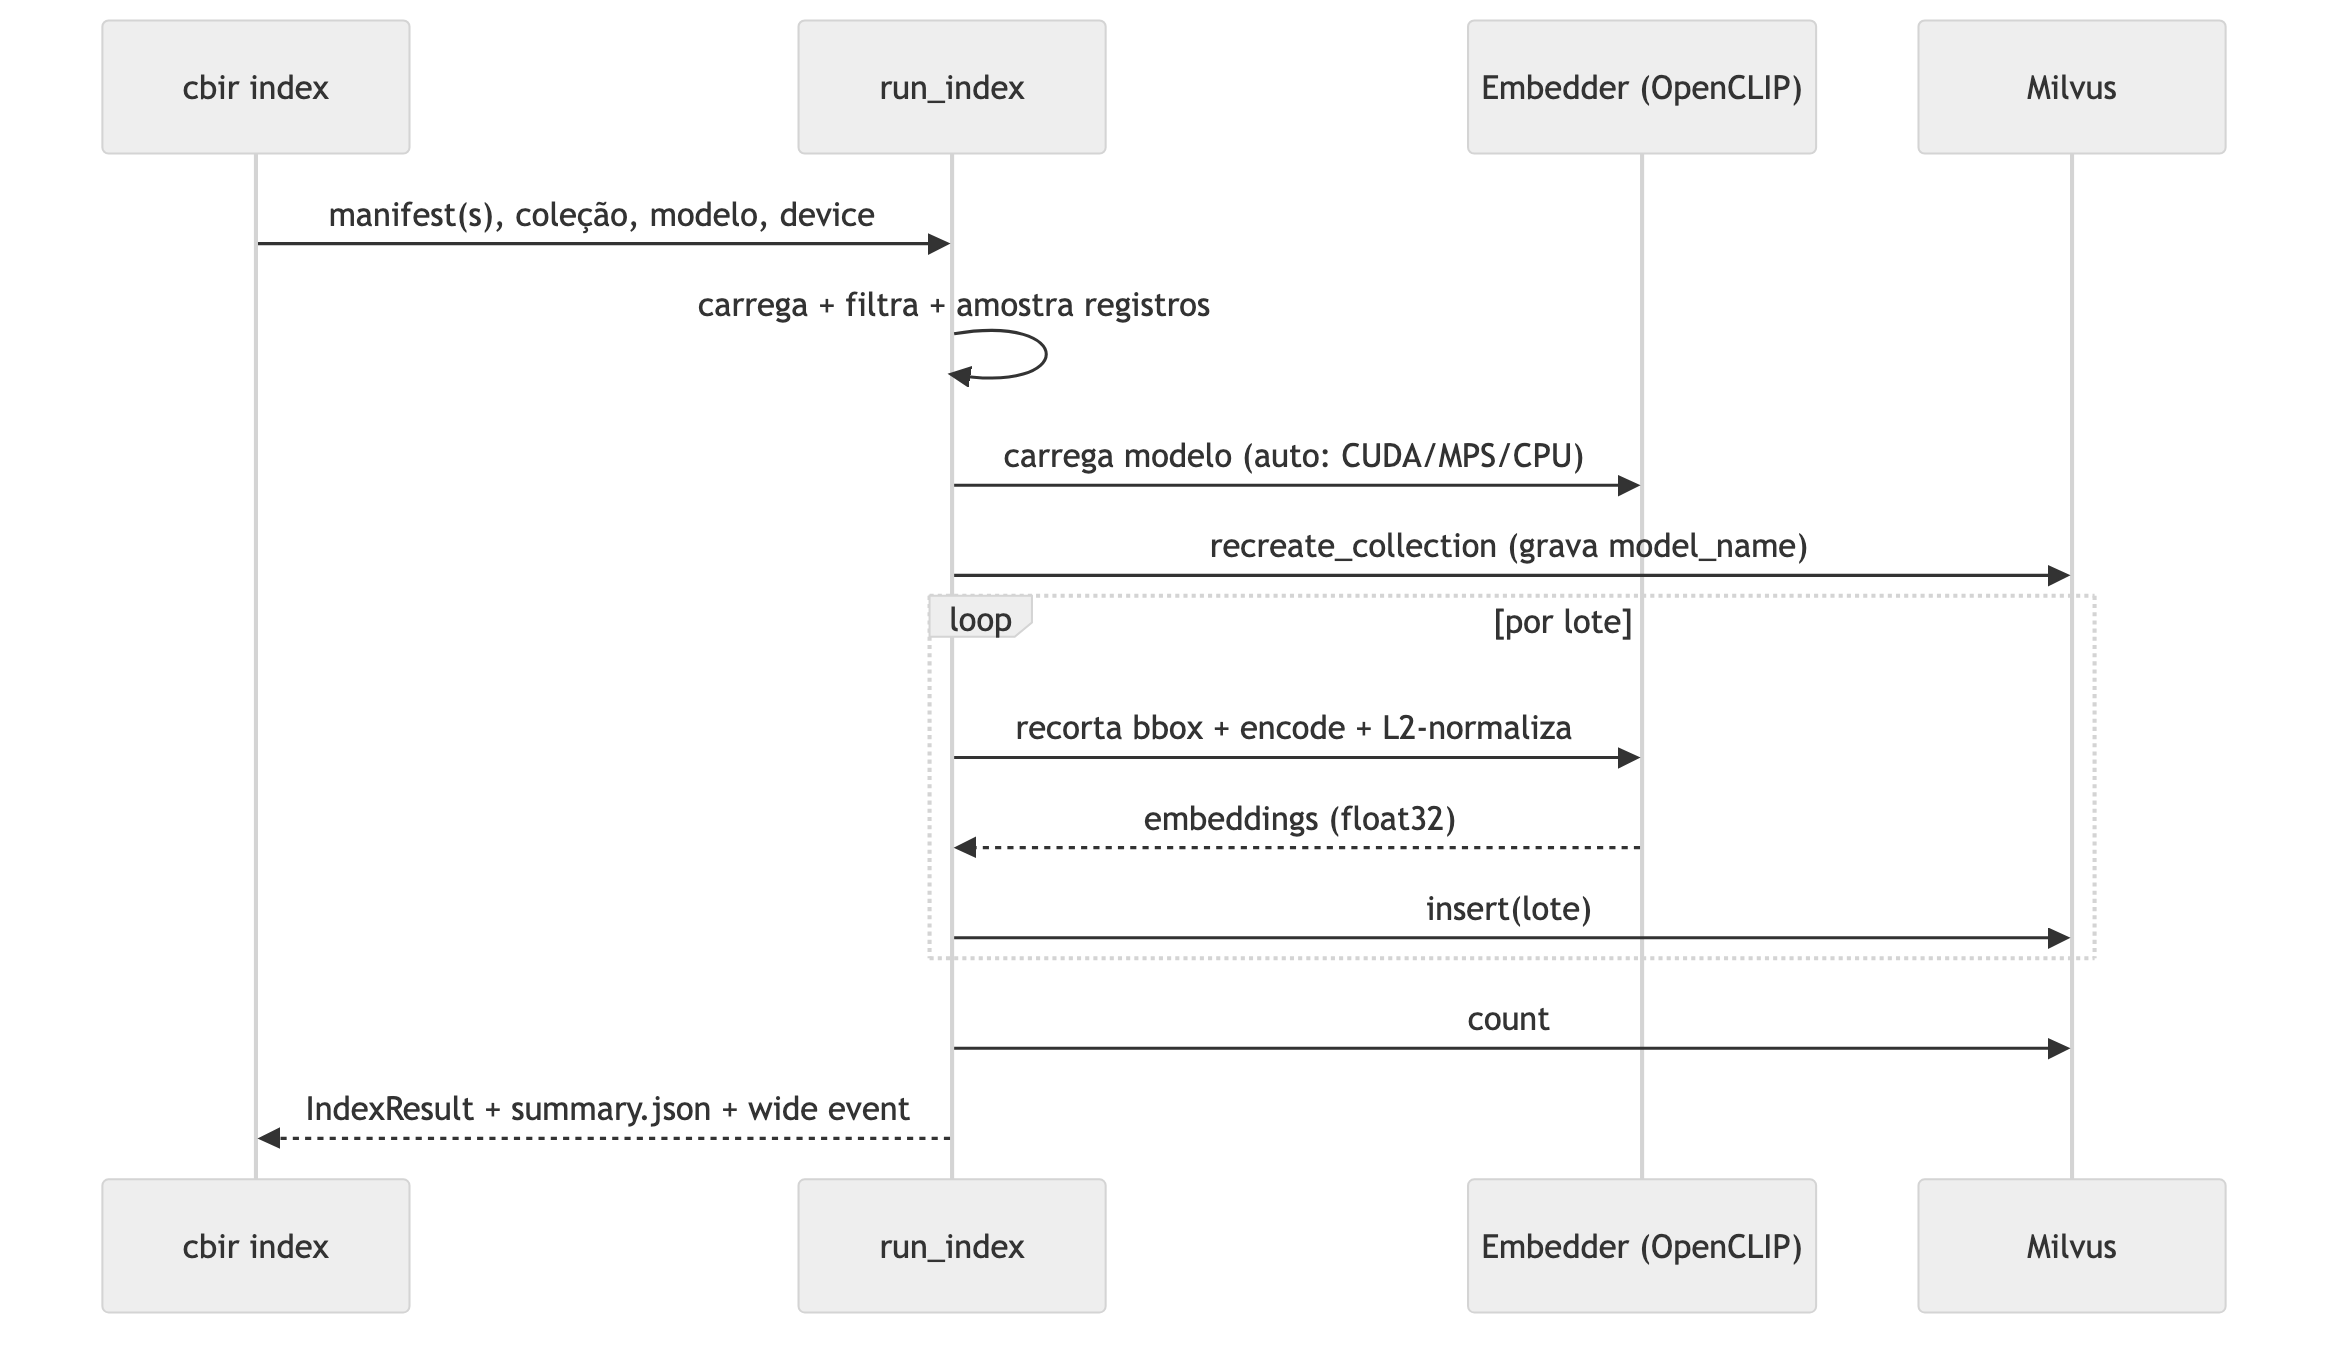
\includegraphics[width=0.92\textwidth]{images/flow_index.png}
  \caption{Fluxo de indexação: \emph{manifest} $\rightarrow$ recorte $\rightarrow$
  \emph{embedding} $\rightarrow$ Milvus, com o modelo gravado na coleção.}
  \label{fig:flow-index}
\end{figure}

\subsection{Fluxo de Consulta}

O fluxo de consulta (Figura~\ref{fig:flow-query}) é o coração da ferramenta:
embeda a imagem com o modelo da coleção, busca os vizinhos, projeta a consulta
no mesmo PCA da galeria e vota a classe.

\begin{figure}[H]
  \centering
  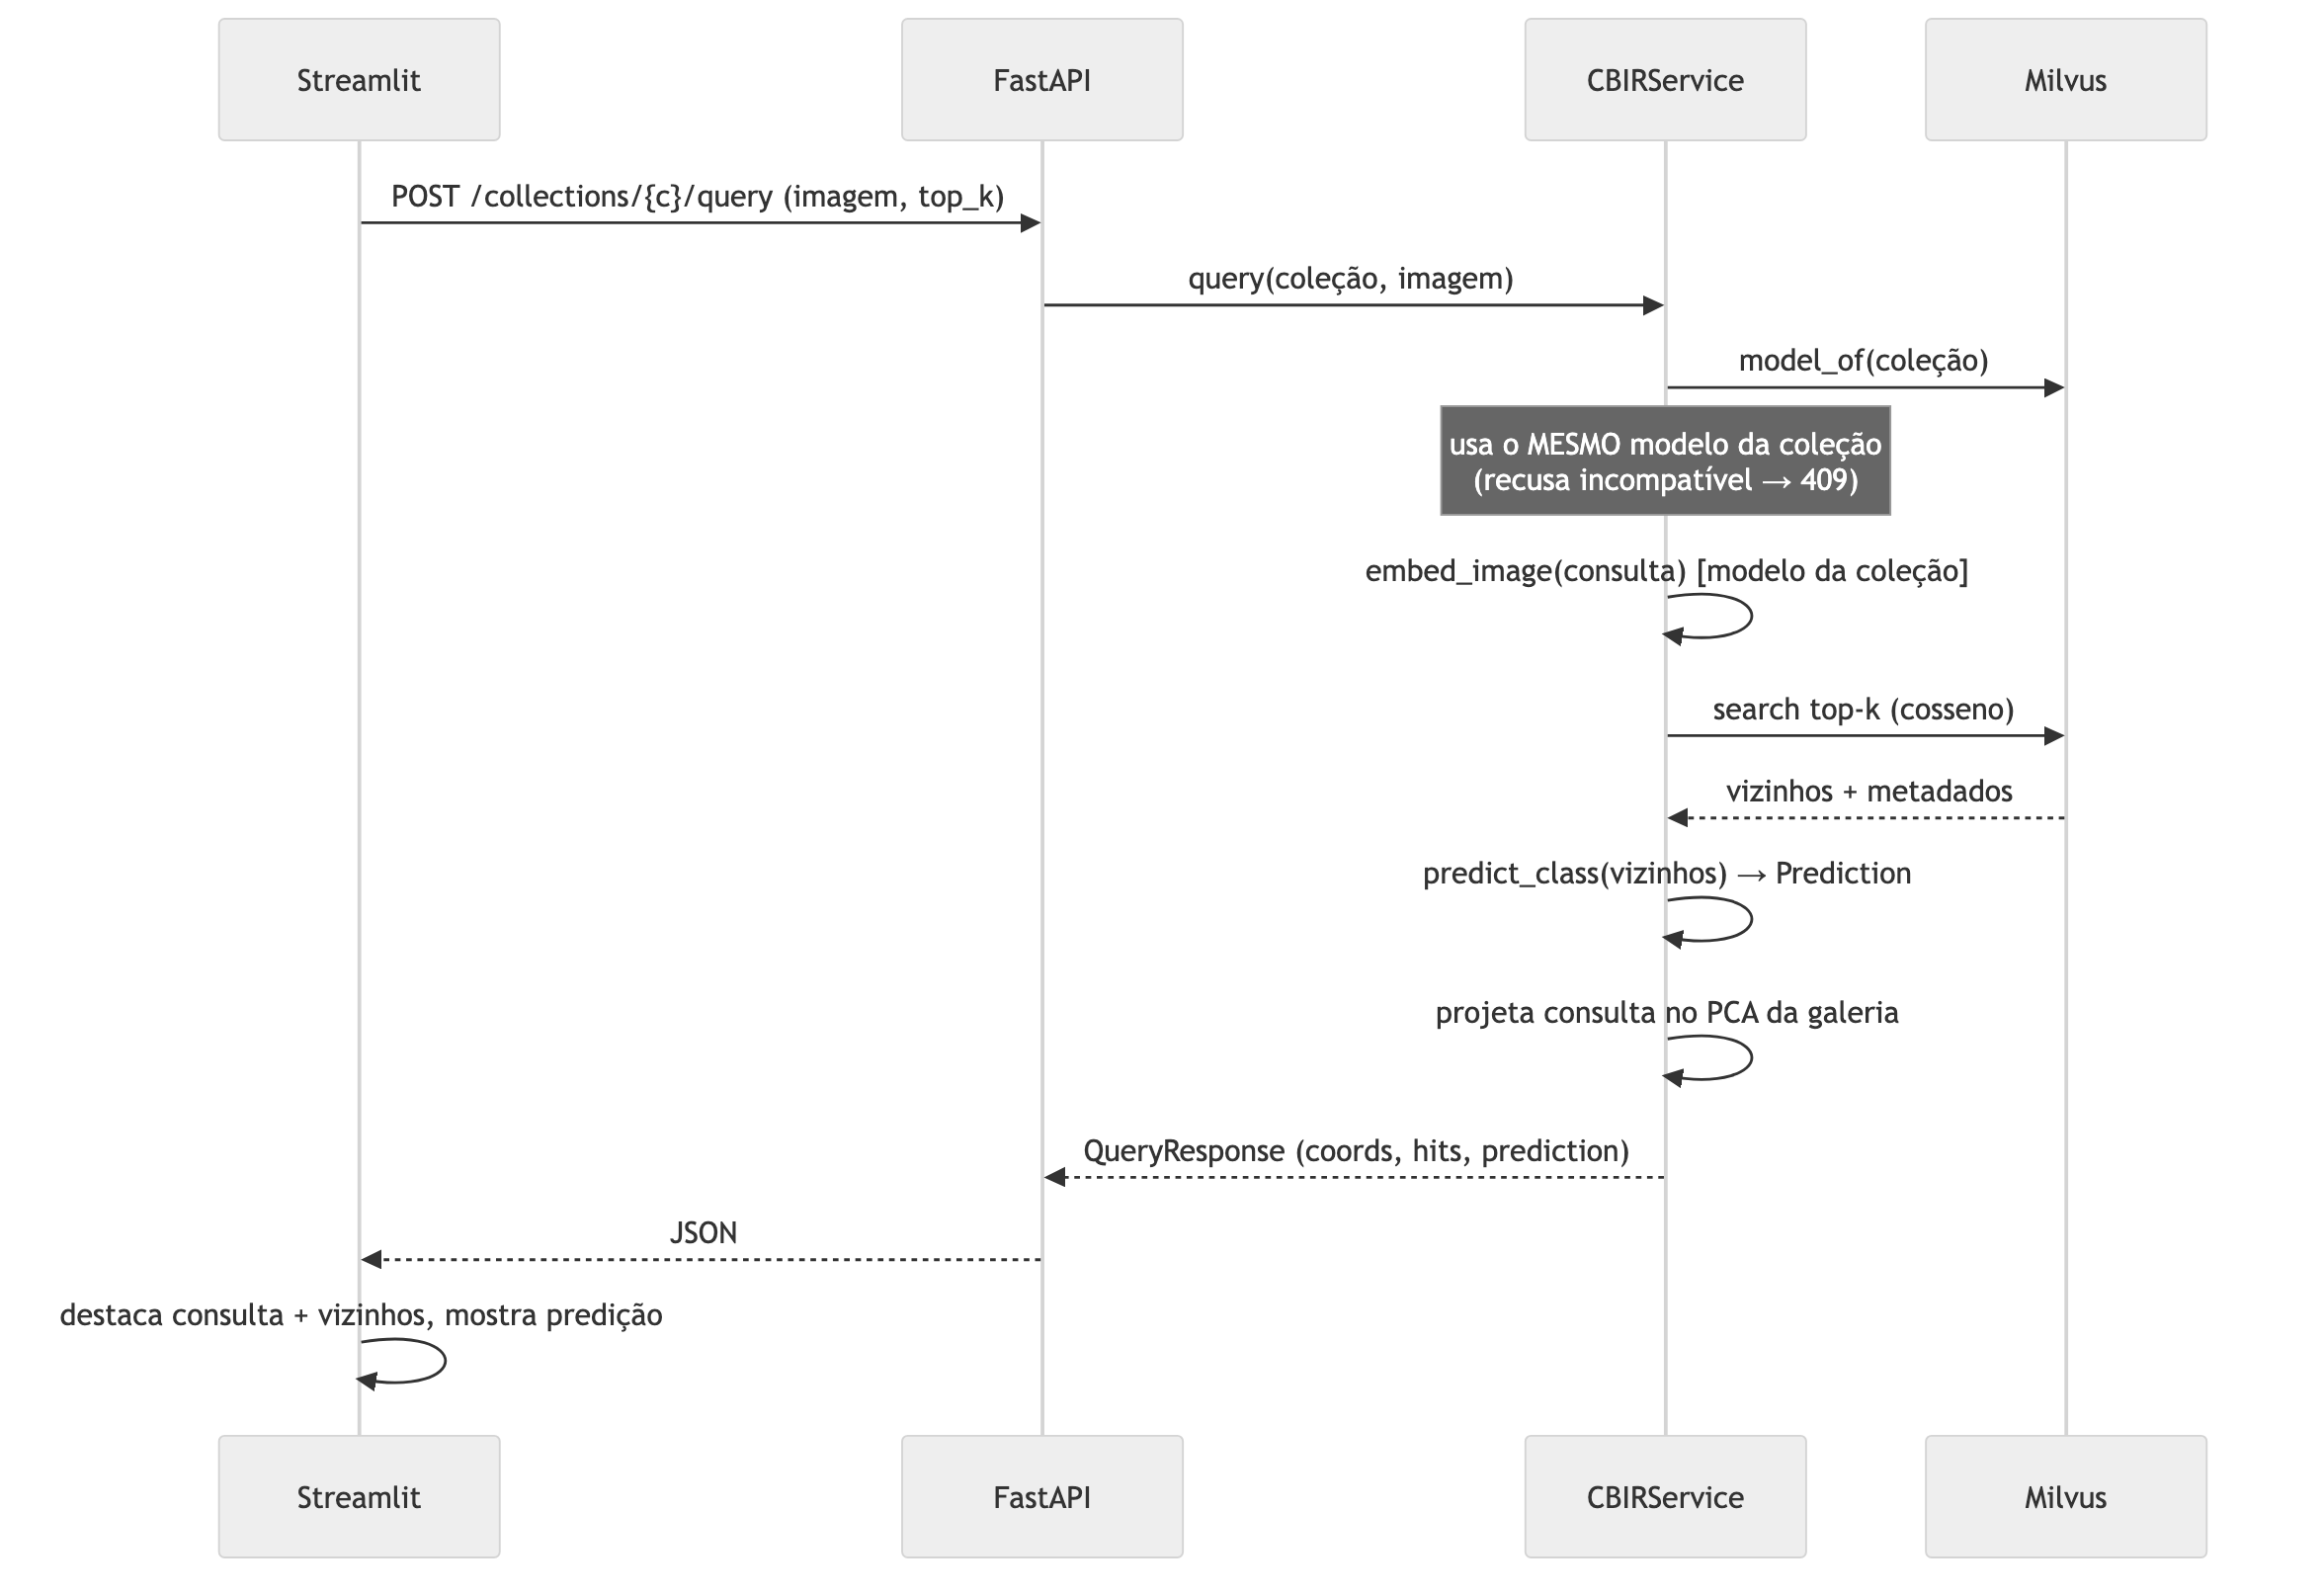
\includegraphics[width=0.95\textwidth]{images/flow_query.png}
  \caption{Fluxo de consulta. A consulta é sempre \emph{embeddada} com o modelo
  da coleção; misturar espaços é recusado com \texttt{409}.}
  \label{fig:flow-query}
\end{figure}

\subsection{Por que PCA (e não t-SNE/UMAP)}

\begin{table}[H]
\centering
\begin{tabular}{@{}p{6.5cm}p{3.5cm}p{4cm}@{}}
\toprule
\textbf{Critério} & \textbf{PCA} & \textbf{t-SNE / UMAP} \\
\midrule
Projetar consulta \textbf{nova} no mesmo espaço & Exato e barato & Sem \texttt{transform} exato \\
Determinismo & Sim & Estocástico \\
Preserva distâncias globais & Sim (linear) & Foco em estrutura local \\
``Onde minha consulta cai vs.\ clusters'' & \textbf{Ideal} & Enganoso \\
\bottomrule
\end{tabular}
\caption{Justificativa da escolha de PCA para a projeção.}
\end{table}

A escolha de PCA é o que torna correta a pergunta central do programa:
\emph{onde esta imagem nova cai em relação aos clusters existentes?}, algo que
exige aplicar exatamente a mesma transformação linear à consulta e à galeria.

\subsection{A garantia de consistência de modelo}

\begin{figure}[H]
  \centering
  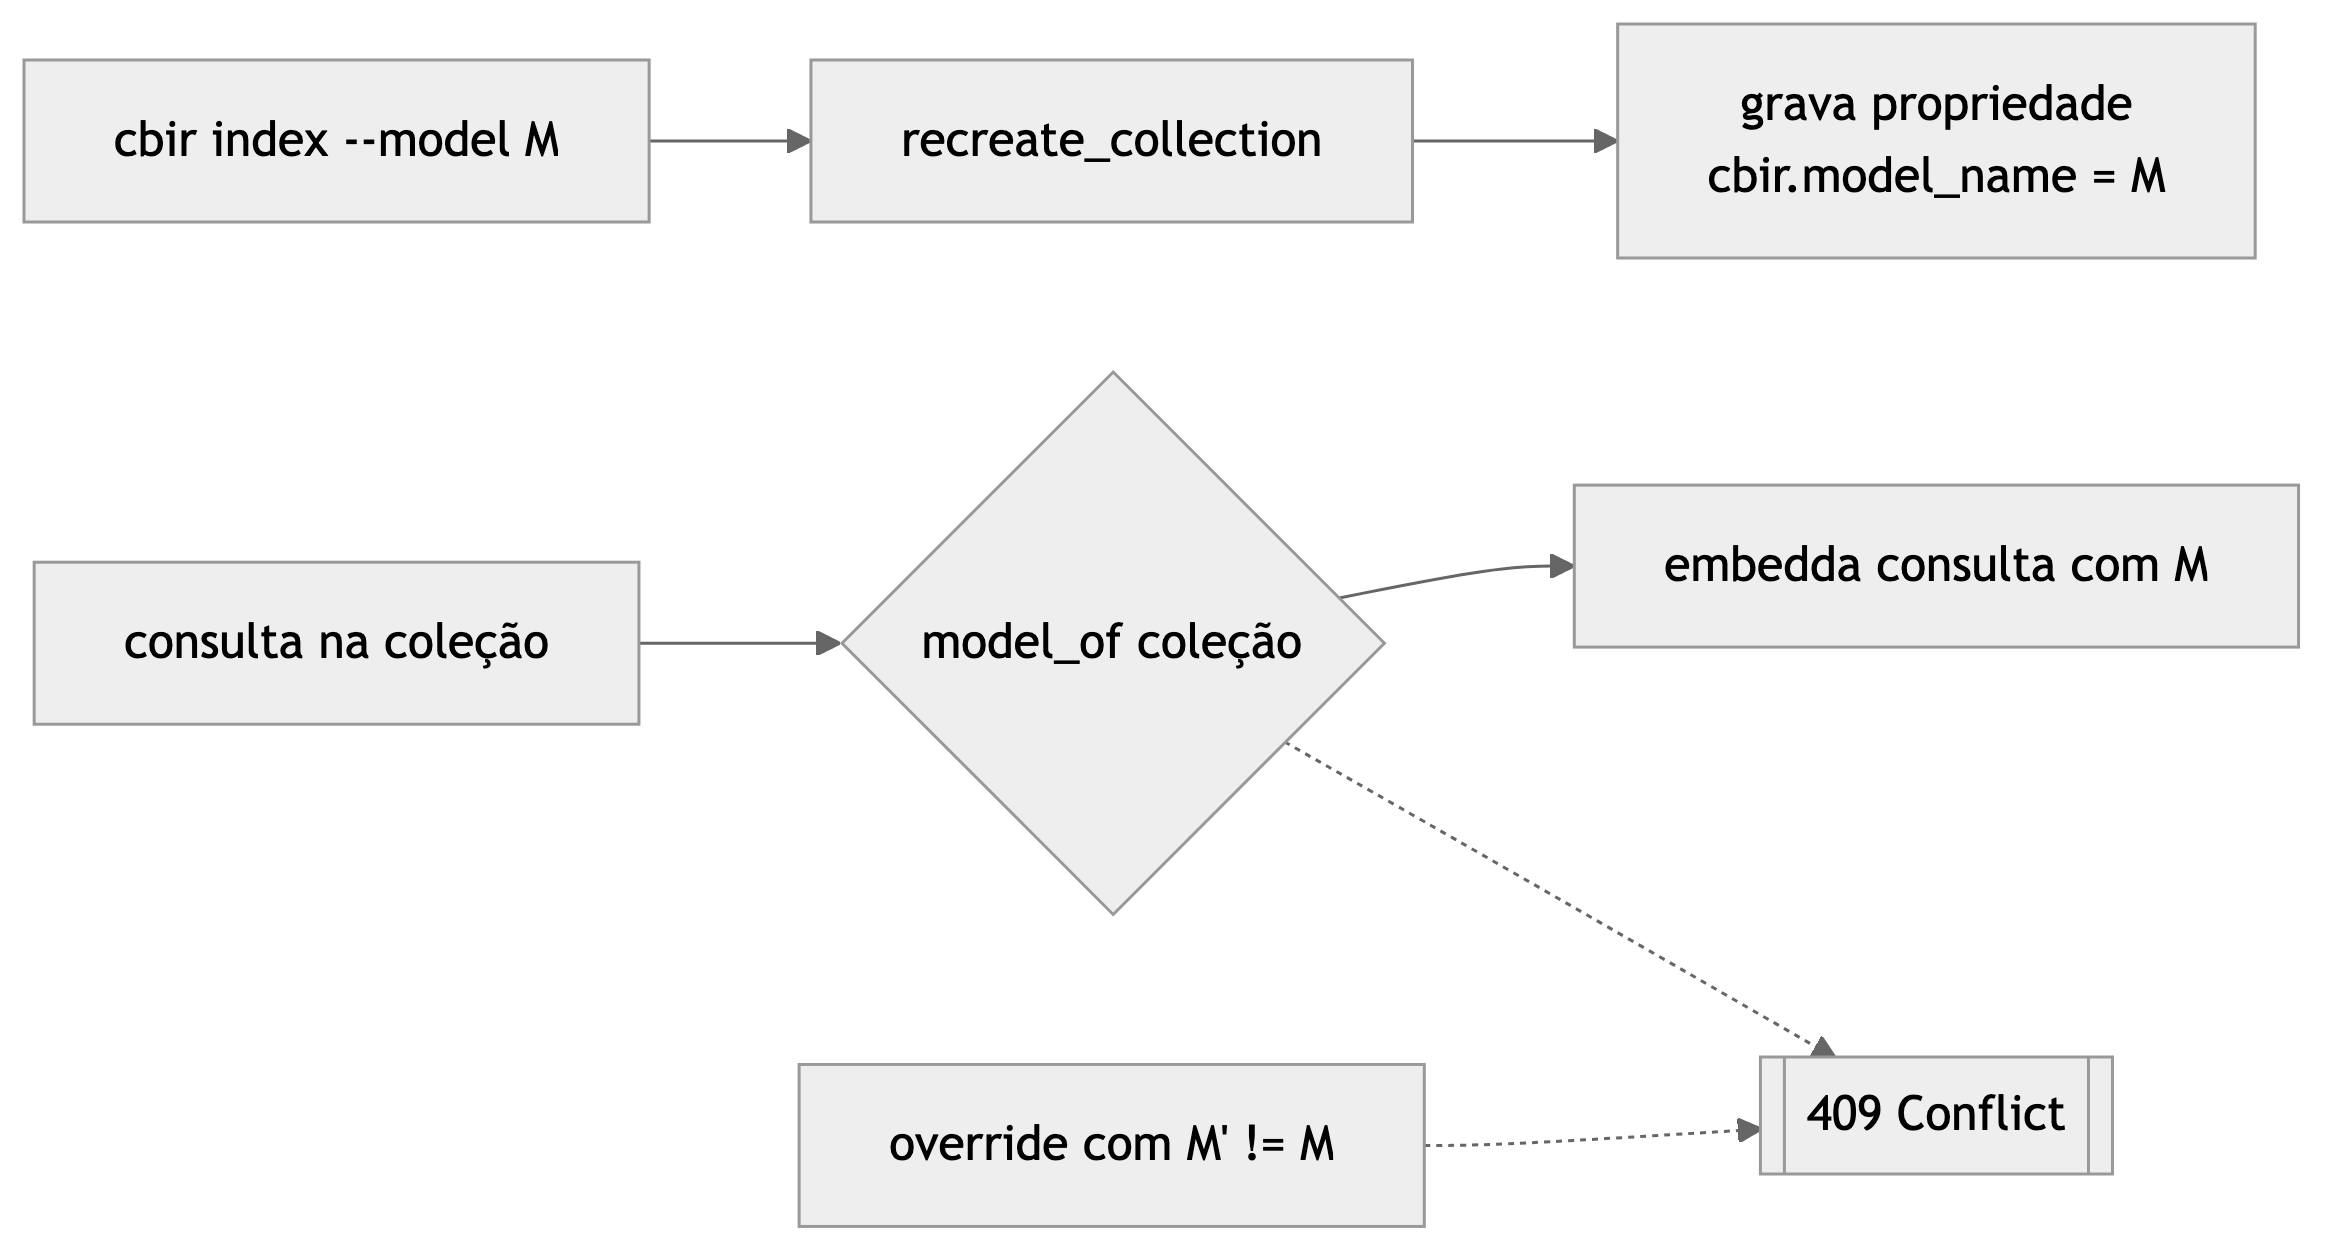
\includegraphics[width=0.85\textwidth]{images/guarantee.png}
  \caption{A coleção grava o modelo que a construiu; a consulta é sempre
  \emph{embeddada} com ele, e qualquer \emph{override} incompatível é recusado.}
  \label{fig:guarantee}
\end{figure}

Um trecho do serviço que implementa a garantia:

\begin{lstlisting}
collection_model = self.model_for_collection(collection)
chosen = model_name or collection_model
if collection_model and model_name and model_name != collection_model:
    raise ModelMismatchError(
        f"Collection {collection!r} was built with {collection_model!r}, "
        f"but the query requested {model_name!r}. "
        "Embeddings would be incomparable."
    )
\end{lstlisting}

\subsection{Resolução de \emph{device}}

O sistema escolhe o melhor acelerador disponível e degrada com elegância
(Figura~\ref{fig:device}), garantindo que o \emph{mesmo} comando rode em
qualquer máquina: CUDA, depois GPU Apple (MPS/Metal), depois CPU
\emph{multi-thread}.

\begin{figure}[H]
  \centering
  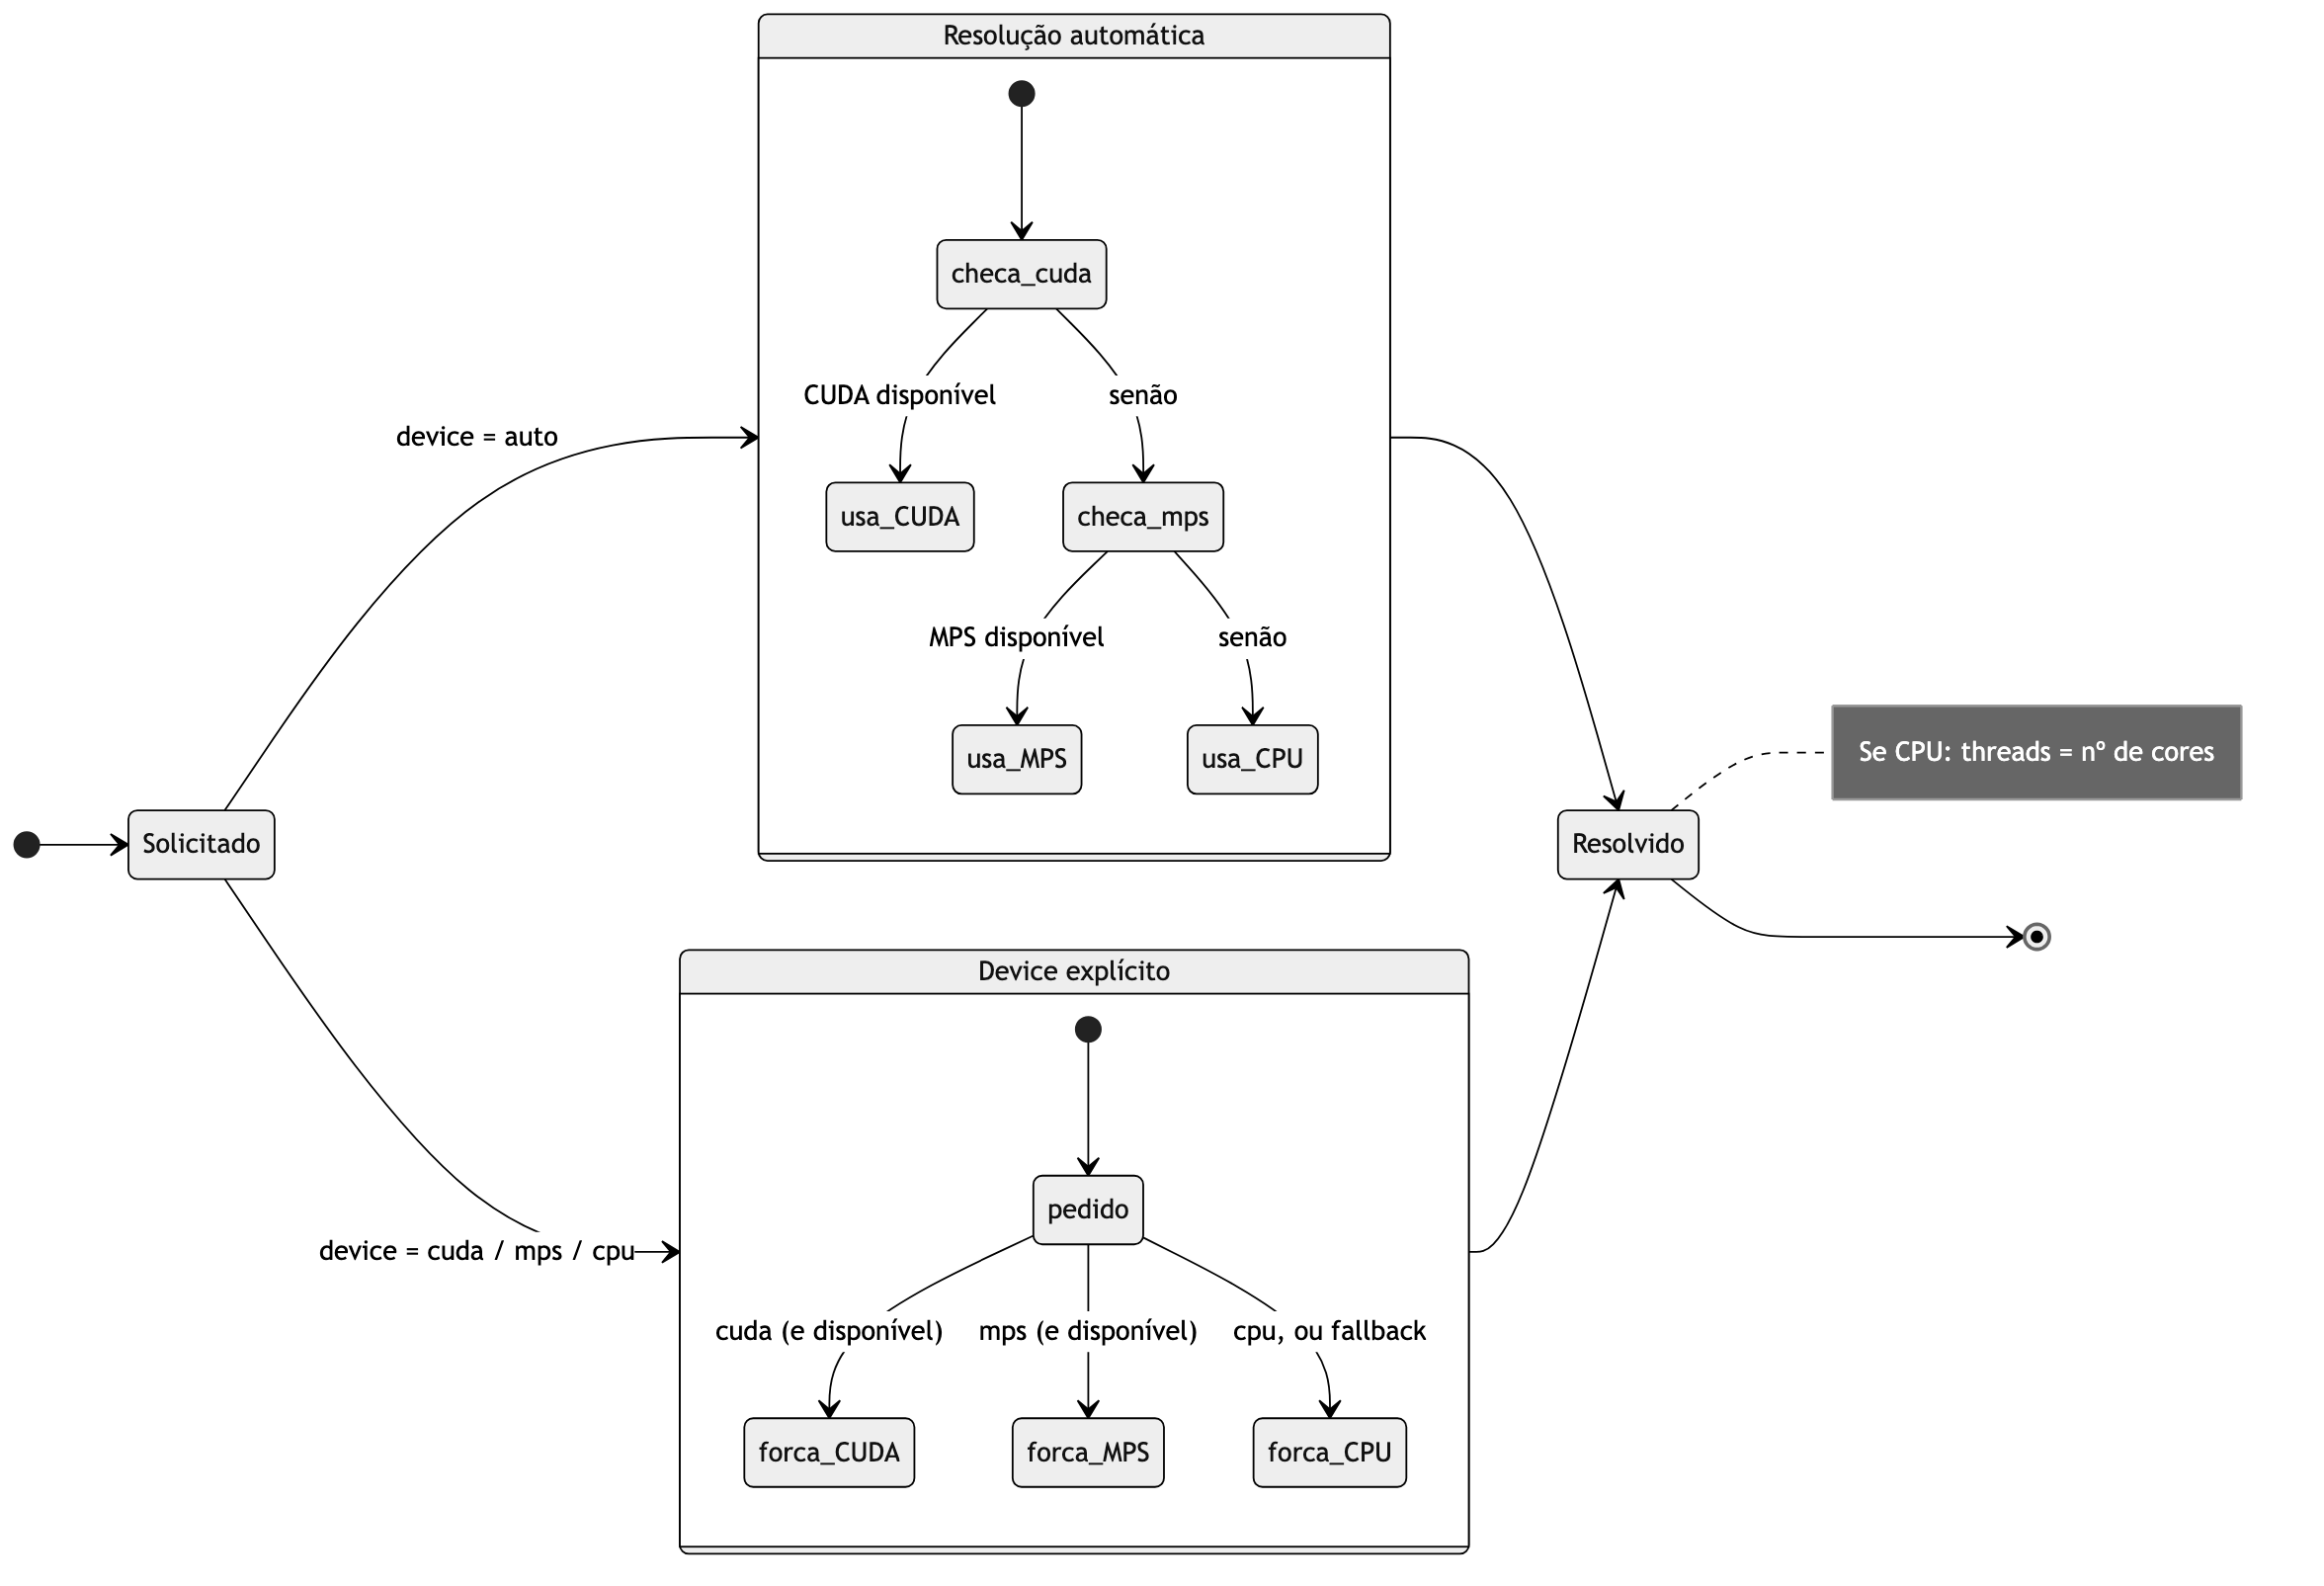
\includegraphics[width=0.8\textwidth]{images/device.png}
  \caption{Máquina de estados da resolução de \emph{device}
  (\texttt{auto} $\rightarrow$ CUDA $\rightarrow$ MPS $\rightarrow$ CPU).}
  \label{fig:device}
\end{figure}

\subsection{Implantação (Docker Compose)}

\begin{figure}[H]
  \centering
  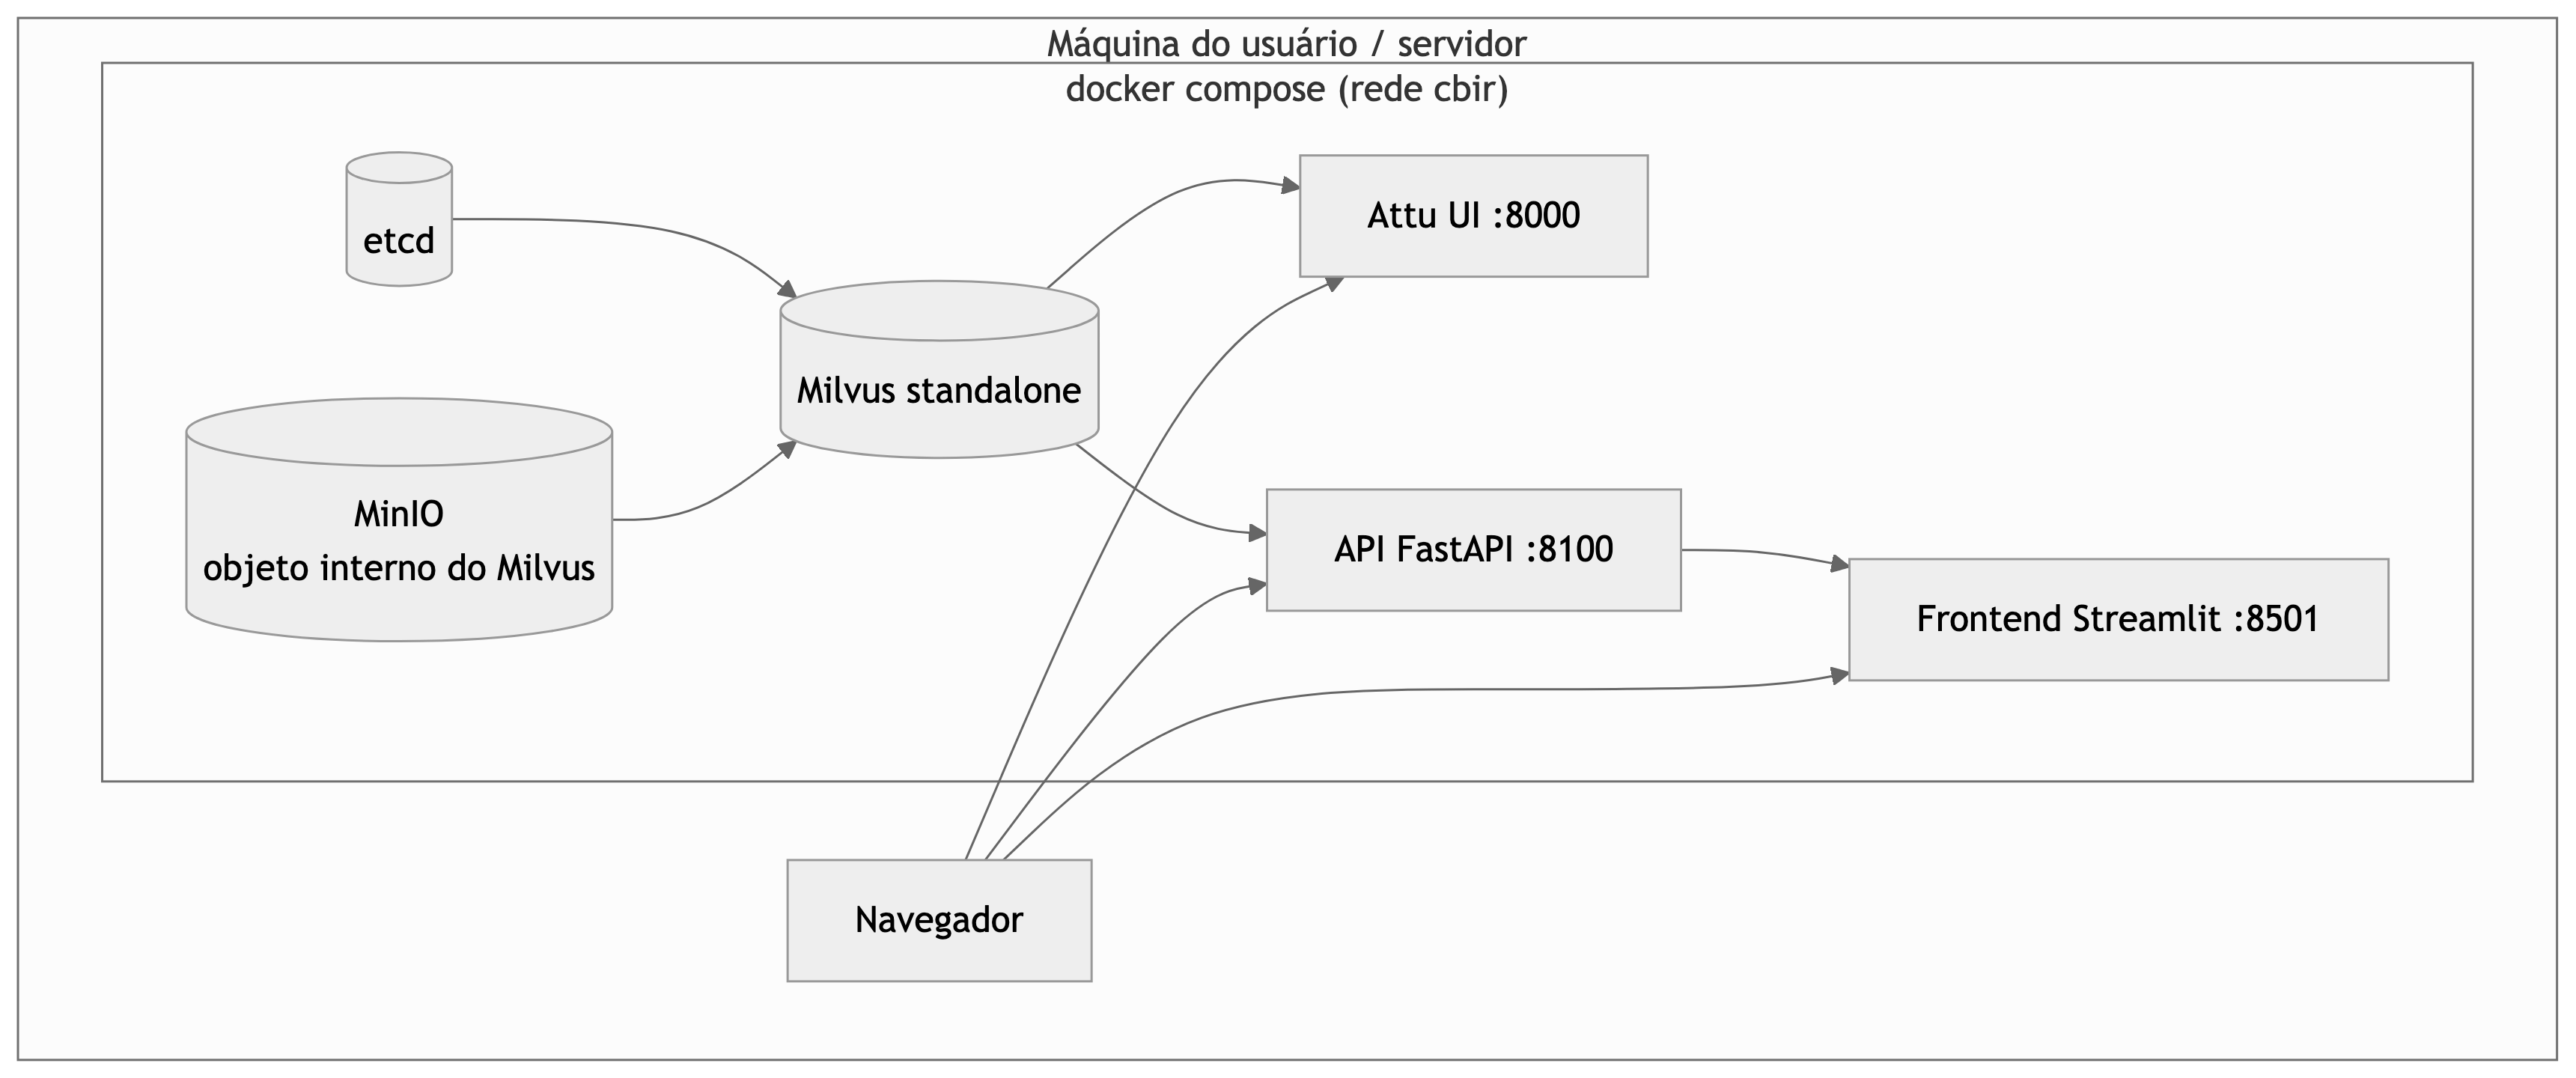
\includegraphics[width=0.95\textwidth]{images/deploy.png}
  \caption{Diagrama de implantação. O perfil padrão sobe apenas o Milvus; o
  perfil \texttt{app} adiciona API e \emph{frontend}.}
  \label{fig:deploy}
\end{figure}

\subsection{Sobre o código}

\begin{table}[H]
\centering
\begin{tabular}{@{}p{4cm}p{10cm}@{}}
\toprule
\textbf{Aspecto} & \textbf{Decisão} \\
\midrule
Linguagem & Python 3.13, gerenciada por \texttt{uv} \\
Contratos de dados & Pydantic v2 (validação nas fronteiras entre camadas) \\
Extração & OpenCLIP; recorte em \emph{runtime}; L2-normalização \\
Banco vetorial & Milvus \emph{standalone} (índice FLAT, métrica cosseno) \\
Projeção & scikit-learn PCA (2D/3D), com degradação graciosa \\
API & FastAPI (endpoints finos sobre o serviço) \\
\emph{Frontend} & Streamlit + Plotly (fala apenas com a API) \\
\emph{Device} & \texttt{auto}: CUDA $\rightarrow$ Apple MPS $\rightarrow$ CPU \emph{multi-thread} \\
Observabilidade & \texttt{logging} \emph{stdlib} com \emph{wide events} \\
Qualidade & \texttt{ruff} (lint), \texttt{mypy} (tipos), \texttt{pytest} (testes) \\
\bottomrule
\end{tabular}
\caption{Principais decisões de implementação.}
\end{table}

\noindent\textbf{Estratégia de comentários:} \emph{docstrings} explicam a
\emph{intenção} e o \emph{porquê} de cada módulo/função; comentários em linha
marcam decisões não óbvias (ex.: por que negar similaridade negativa no voto,
por que PCA e não UMAP). Código óbvio não é comentado.

\medskip
\noindent\textbf{Estratégia de testes:} o \emph{backend} é puro e testado sem
Milvus/torch (projeção, KNN, \emph{manifest}, modelos); a API é testada com um
serviço falso, verificando inclusive a garantia de consistência de modelo
(\texttt{409}). São 30 testes, executados com:

\begin{lstlisting}[language=bash]
uv run ruff check cbir/ tests/   # lint
uv run mypy cbir/                # tipos
uv run pytest                    # testes
\end{lstlisting}

% Manual
\section{Manual de Utilização}

O manual cobre os dois tipos de usuário visados: quem quer \textbf{rodar a
demo} rapidamente e quem quer \textbf{indexar dados próprios}.

\subsection{Instalação}

\begin{lstlisting}[language=bash]
uv sync                 # instala dependencias
docker compose up -d    # sobe Milvus (etcd + minio + milvus + Attu)
# aguarde o Milvus ficar "healthy" (docker compose ps)
\end{lstlisting}

\subsection{Tarefa A: Rodar a demonstração (sem GPU, sem baixar modelo)}

\begin{lstlisting}[language=bash]
uv run cbir seed --collection cbir_sample \
    --parquet cbir/sample_data/embeddings.parquet
uv run cbir api    # terminal 1: API em :8100
uv run cbir app    # terminal 2: frontend em :8501
# abra http://localhost:8501, escolha "cbir_sample" e envie um recorte
\end{lstlisting}

\noindent\textbf{Exceções e problemas comuns:}
\begin{itemize}
  \item \emph{``API not reachable''}: confirme que \texttt{cbir api} está
  rodando e a porta 8100 está livre.
  \item \emph{Gráfico vazio}: rode \texttt{cbir seed} antes de abrir o app; a
  coleção precisa existir.
\end{itemize}

\subsection{Tarefa B: Indexar dados próprios}

\begin{lstlisting}[language=bash]
uv run cbir index --manifest <caminho> --collection <nome> \
    --model openclip-vit-b-32 --device auto
# (opcional) snapshot reproduzivel:
uv run cbir export --collection <nome> --model openclip-vit-b-32
\end{lstlisting}

\noindent\textbf{Exceções e problemas comuns:}
\begin{itemize}
  \item \emph{``No records selected''}: revise \texttt{--split} /
  \texttt{--benchmark-only} / \texttt{--per-class}.
  \item \emph{Consulta recusada com \texttt{409}}: a coleção foi construída com
  outro modelo; use o modelo da coleção.
\end{itemize}

\subsection{Referência de comandos e endpoints}

\begin{table}[H]
\centering
\begin{tabular}{@{}p{2.5cm}p{11.5cm}@{}}
\toprule
\textbf{Comando} & \textbf{O que faz} \\
\midrule
\texttt{cbir sample} & Constrói o \emph{dataset} de amostra comitável (recortes + \emph{manifest}) \\
\texttt{cbir index} & Extrai \emph{embeddings} de um \emph{manifest} e indexa no Milvus \\
\texttt{cbir export} & Exporta os \emph{embeddings} de uma coleção para um cache Parquet \\
\texttt{cbir seed} & Reconstrói uma coleção a partir de um cache Parquet (sem modelo) \\
\texttt{cbir api} & Sobe o serviço FastAPI \\
\texttt{cbir app} & Sobe o \emph{frontend} Streamlit \\
\bottomrule
\end{tabular}
\caption{Comandos da CLI.}
\end{table}

\begin{table}[H]
\centering
\begin{tabular}{@{}llp{7.5cm}@{}}
\toprule
\textbf{Método} & \textbf{Rota} & \textbf{Função} \\
\midrule
GET  & \texttt{/health} & Verificação de vida \\
GET  & \texttt{/models} & Modelos de \emph{embedding} disponíveis \\
GET  & \texttt{/collections} & Coleções indexadas + modelo + contagem \\
GET  & \texttt{/collections/\{n\}/project} & Coordenadas PCA da galeria (2D/3D) \\
POST & \texttt{/collections/\{n\}/query} & Imagem $\rightarrow$ vizinhos + predição KNN + coords \\
GET  & \texttt{/crop} & Serve um recorte por caminho de \emph{manifest} \\
\bottomrule
\end{tabular}
\caption{Endpoints da API.}
\end{table}

% Verificação
\section{Verificação}

O sistema foi validado de ponta a ponta na máquina de desenvolvimento
(Apple Silicon, \emph{device} \texttt{mps}).

\begin{table}[H]
\centering
\begin{tabular}{@{}p{8.5cm}p{5.5cm}@{}}
\toprule
\textbf{Verificação} & \textbf{Resultado} \\
\midrule
Indexação da amostra (160 recortes, 4 classes) & 160 itens em $\approx$29\,s (MPS) \\
Projeção PCA 2D/3D da galeria & 160 pontos; \texttt{transform} exato \\
Consulta ponta a ponta (upload $\rightarrow$ busca $\rightarrow$ KNN $\rightarrow$ projeção) & Predição coerente com confiança \\
Garantia de consistência de modelo & Recusa (\texttt{409}) confirmada em teste \\
\texttt{ruff} / \texttt{mypy} / \texttt{pytest} & Limpo / limpo / 30 testes passando \\
Reconstrução via cache (\texttt{seed}) & Coleção recriada em $\approx$3\,s sem GPU \\
\bottomrule
\end{tabular}
\caption{Resultados da verificação de ponta a ponta.}
\end{table}

\section{Conclusão e Trabalhos Futuros}

O programa entrega um sistema CBIR funcional e reproduzível, com três camadas
bem separadas, uma garantia explícita de consistência de modelo, e uma interface
visual que torna concreta a pergunta central da pesquisa: \emph{uma imagem de
classe A se posiciona perto de outras da classe A e longe das demais?} Como
trabalhos futuros, destacam-se: (i) a comparação sistemática entre modelos de
\emph{embedding}; (ii) o uso de \emph{embeddings} derivados de um detector
treinado no domínio; e (iii) a avaliação quantitativa da confiabilidade dos
limiares de similaridade para rotulagem automática, que é o objeto da
dissertação.

\end{document}
